%\documentclass[letterpaper, 10 pt, conference]{ieeeconf}  % Comment this line out if you need a4paper

\documentclass[a4paper, 10pt, conference]{ieeeconf}      % Use this line for a4 paper

\IEEEoverridecommandlockouts                              % This command is only needed if 
                                                          % you want to use the \thanks command

\overrideIEEEmargins                                      % Needed to meet printer requirements.

%In case you encounter the following error:
%Error 1010 The PDF file may be corrupt (unable to open PDF file) OR
%Error 1000 An error occurred while parsing a contents stream. Unable to analyze the PDF file.
%This is a known problem with pdfLaTeX conversion filter. The file cannot be opened with acrobat reader
%Please use one of the alternatives below to circumvent this error by uncommenting one or the other
%\pdfobjcompresslevel=0
%\pdfminorversion=4

% See the \addtolength command later in the file to balance the column lengths
% on the last page of the document

% The following packages can be found on http:\\www.ctan.org
%\usepackage{graphics} % for pdf, bitmapped graphics files
%\usepackage{epsfig} % for postscript graphics files
%\usepackage{mathptmx} % assumes new font selection scheme installed
%\usepackage{times} % assumes new font selection scheme installed
%\usepackage{amsmath} % assumes amsmath package installed
%\usepackage{amssymb}  % assumes amsmath package installed

\usepackage[hidelinks]{hyperref}
\usepackage{amsmath}
\usepackage{graphicx}
\usepackage{caption}


\title{\LARGE \bf
Mobile Robot Systems Mini Project 5
}


\author{Sam Sully (sjs252), Paul Durbaba (pd452), Luke Dunsmore (ldd25)}


\begin{document}

\maketitle

\section{Introduction}
Our project seeks to control a number of robots in a collaborative multi-robot system in order to cover a map in the shortest time. In order to do this the robots will need to localise so that they can report their positions, and thus covered areas. We implement the collaborative localisation strategy presented in Dr Prorok's thesis~\cite{prorok} and compare it with the simpler particle filter implemented in exercise 1 of the Mobile Robots System course.
\section{Localisation}
This section of the project was developed by Sam Sully (sjs252). The approach used was a combination of the sensor-based particle filter used in exercise 1 and the range and bearing approach presented in Dr Prorok's thesis~\cite{prorok}.
\subsection{Particle Filter}
The particle filter works by randomly picking samples (particles) from a proposal distribution and then computing the probability that each particle is correct based on measurements from the robot's sensors. We then re-sample the particles, replacing the less likely ones with more likely ones.
\subsection{LIDAR}
Our approach used a known map, the range sensors measurements from the robot's LIDAR and the range and bearing measurements between robots. The weight of the robot is first calculated using the range sensor measurements using a Gaussian measurement model. The weight is given by the below formula:
\[
	w_i = \prod_{s_{j} \in \mathrm{Sensors}}\Phi(R(i,j), s_{ij}, \sigma^2)
\]
where $w_i$ is the weight of particle $i$, $s_{ij}$ is the distance recorded by sensor $j$ on the robot, $\Phi(x,\mu,\sigma)$ is the Gaussian PDF with mean $\mu$ and standard deviation $\sigma$ and $R(i,j)$ is the ray traced distance from particle $i$ in the direction of sensor $j$.

This can effectively be summarised as the product of the Gaussian PDF for each sensor where the mean is the sensor's observed value and the input to the PDF is the raytraced distance from that particle.
\subsection{Range \& Bearing}
We then refine the weight if there are any other robots in range and line-of-sight (these robots are referred to as the neighbours, the set $N_i$ represents robot $i$'s neighbours.). To do this we compute a second weight, $\bar{w_i}$ using the below formula:
\[
	\bar{w_i} = \prod_{r_j \in N_i}\sum_{p_k \in r_j}\Phi\left(
	\begin{bmatrix}
		D_i(p_k)\\
		\Theta_i(p_k)
	\end{bmatrix},
	\begin{bmatrix}
		d_j\\
		\theta_j
	\end{bmatrix},
	\xi
	\right)\cdot w_{p_k}
\]
where $p_k$ ranges over the set of particles from robot $r_j$, $d_j$ is the received distance between this robot and robot $r_j$, $\theta_j$ is the received bearing of this robot from $r_j$, $D_i(p_k)$ is the distance between the particle $i$ on this robot and the particle $p_k$ from the other robot, $\Theta_i(p_k)$ is the bearing between the particle $i$ and the particle $p_k$ on the other robot, $\xi$ is the covariance matrix and $w_{p_k}$ is the weight of the particle $p_k$. I have omitted normalisation factors.

This can be explained as taking the product of the sums of the bivariate Gaussian PDF for each particle in each robot in range where the means are the range reported from that robot and the bearing reported from that robot and the input to the PDF is the calculated values of range and bearing based on that particle's pose and the local particle's pose.

We then take these two quantities, $w_i$ and $\bar{w_i}$ and multiply them together to get the final weight.
\subsection{Performance}
We will now compare the performance of the collaborative localisation and the non-collaborative approach. To do this we created a test environment where two robots were already well-localised and one was not, this was done because the system does not perform well in an environment where all robots are initially poorly localised due to rumour propagation. Figure~\ref{fig:loca1} shows the localisation error over time with the collaborative approach while figure~\ref{fig:loca2} shows the error for the standard (non-collaborative) approach. As can be clearly seen the collaborative approach yields a much faster convergence and a lower error following convergence.
\begin{figure}
	\centering
	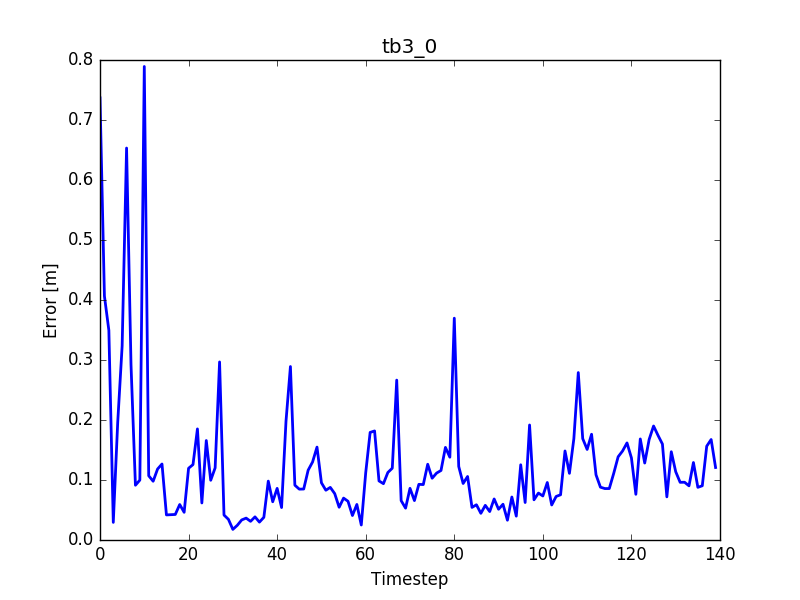
\includegraphics[width=\columnwidth]{figure_l1.png}
	\caption{Error of localisation estimation over time using collaborative approach.}
	\label{fig:loca1}
\end{figure}
\begin{figure}
	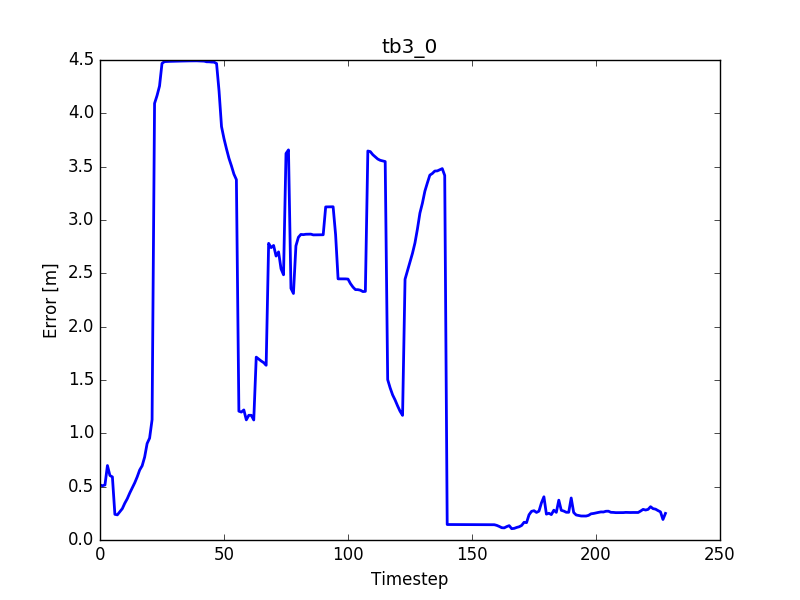
\includegraphics[width=\columnwidth]{figure_l2.png}
	\caption{Error of localisation estimation over time using standard approach.}
	\label{fig:loca2}
\end{figure}
I tried varying the sensor noise and noticed a decrease in performance as noise was increased as one might expect. Additionally, increasing robot density improves the performance only in the case where most of the robots are well localised initially, otherwise we see rumour propagation issues as previously noted. It was difficult to gather useful data on robot density as Gazebo struggles with more than a small number of robots.

\section{Centralised Navigation}
This section of the project was developed by Luke Dunsmore (ldd25). The focus was on issuing movement instructions to the robots from a centralised server such that the robots cover as much of the world as possible in the shortest amount of time.

\subsection{Partitioning the world}
The benefit of having centralised control is that you can make a fully informed decision about how best to direct the robots. Our approach was to allow the robots to move freely in the world until they were able to somewhat accurately localise themselves. Once they knew where they were, we could assign each robot a portion of the world that it would be their responsibility to cover. We divide the world into regions using the DARP algorithm ~\cite{darp}.

\subsection{DARP}
\label{section:darp}

DARP, which is an acronym for Divide Areas based on initial Robot Positions, takes a world represented as a map of cells, and iteratively assigns the cells to robots. For each robot, there is an evaluation matrix, $E$, which is initially filled with the distance from the robot to each cell in the world. At each iteration after these matrices have been updated, each cell is assigned to a robot as follows:
\begin{equation*}
	A_{x, y} = \underset{i \in {\{1,\hdots,n_r\}}}{\mathrm{argmin}} E_{i|x,y}, \forall(x, y) \in \mathcal{L}
\end{equation*}
where $n_r$ is the number of robots, $E_i$ is the evaluation matrix for the $i$th robot, and $\mathcal{L}$ is the cellular representation of the world. The aim of the algorithm is to divide the world into $n_r$ regions, $L_i$, such that the following conditions hold:
\begin{enumerate}
	\item $L_i \cap L_j = \phi , \forall i, j \in 1, \hdots, n_r, i \neq j$
	\item $L_1\cup L_2 \cup \cdots \cup L_{n_r} = \mathcal{L}$
	\item $|L_1| \approx |L_2| \cdots \approx |L_{n_r}|$
	\item $L_i$ is connected $\forall i \in 1, \hdots, n_r$
	\item $\chi_i(t_0) \in L_i$
\end{enumerate}
where $\chi_i(t_0)$ is the initial location of robot $i$. Each region is determined from the assignments, $A$, as follows:
\begin{equation*}
L_i = \{(x, y) \in \mathcal{L} : A(x, y)=i\}, \forall i \in 1, \hdots, \mathcal{L}
\end{equation*}
Of the conditions listed above, (1) and (2) are taken care of by the fact that the argmin function assigns exactly one robot to each cell. Condition (5) can be handled by allowing a 0 value for cell $(i, j)$ of $E_k$ if and only if robot $k$ is in cell $(i, j)$.

To satisfy condition (3), we iteratively adjust the values in the evaluation matrix. To ensure the regions are of roughly equal sizes, we decrease the values in $E_i$ if $|L_i| < f$, where $f$ is the size of a region obtained through a perfectly equal split of the world, and we increase the values in $E_i$ if $|L_i| > f$.

For condition (4), for each region, $R_i$, that is not continuous we create a matrix, $C_i$, where cells that are close to the section of $R_i$ that the robot is in, and far from the sections that the robot is not in score highly, and cells that are far from the robot's section and close to the other sections score lowly. The evaluation matrix $E_i$ is then multiplied element-wise by $C_i$.

An example assignment of a world to 4 robots is shown in figure~\ref{fig:darp}.

\begin{figure}
	\centering
	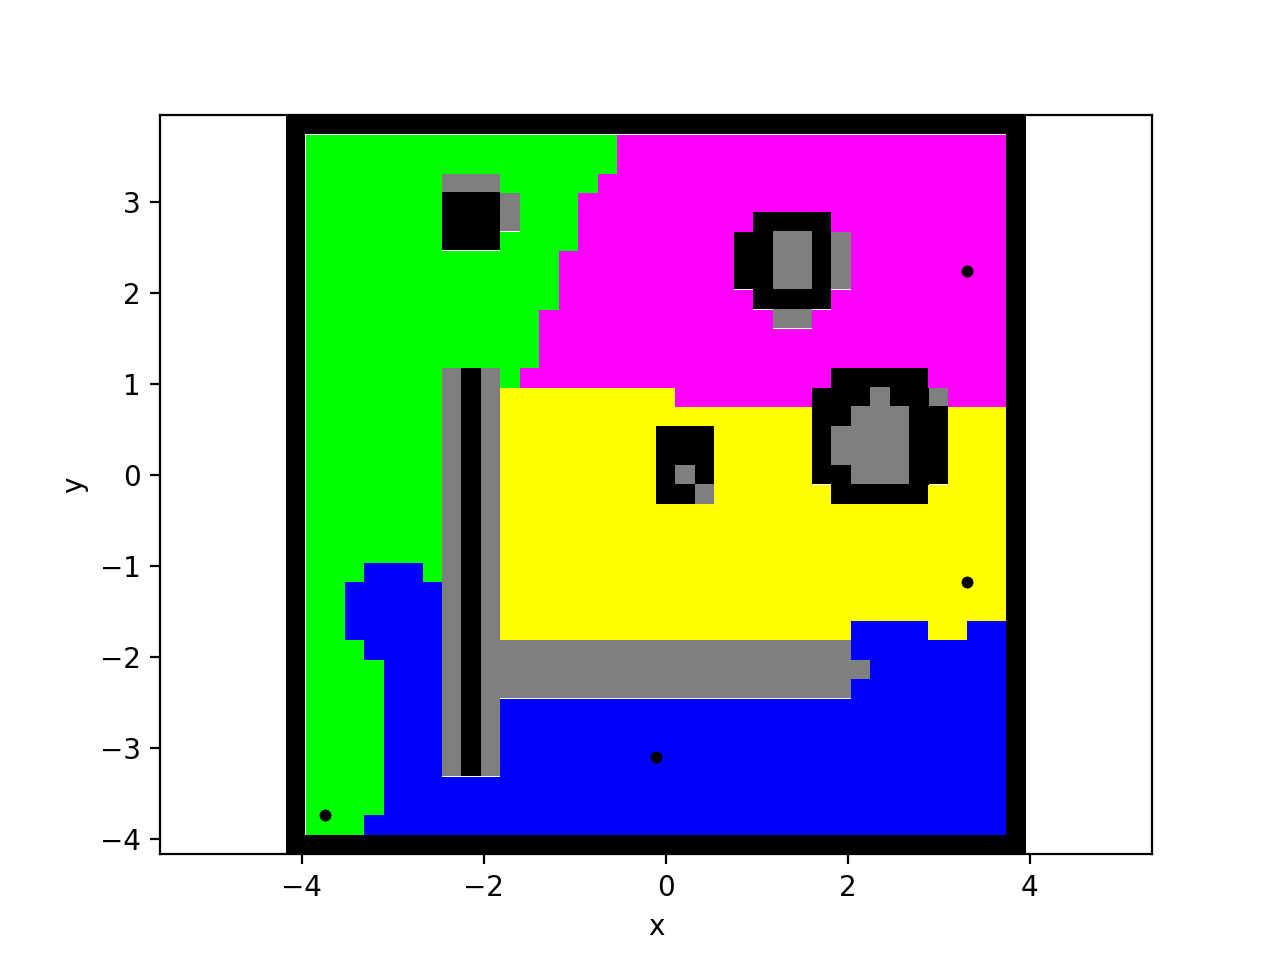
\includegraphics[width=\columnwidth]{figure_darp.png}
	\caption{Division of world into 4 regions.}
	\label{fig:darp}
\end{figure}
   
\subsection{Path Planning}
After each robot is assigned to a region, we calculate a path that it must travel along within its region such that it covers the whole region in the shortest time possible. We aim to do this by minimising the amount of duplicate coverage in the region - that is, covering a part of the region twice, before every part of the region has been covered once. Before running the DARP algorithm, explained in section~\ref{section:darp}, we divide the world into square cells with edges of length double the diameter of the robots. This allows a robot to cover the cell with a single pass in both directions.

After running the DARP algorithm and obtaining a region for each robot to cover, we create a minimum spanning tree that connects the centres of every cell in the region. Since the distance between any two cells are equal, any spanning tree will be a minimum one, so we have freedom to choose edges that will maximise the amount of amount of continuous straight lines in order to minimise time spent turning, which is time not covering new ground. Figure~\ref{fig:mst} shows spanning trees for the three regions.

To generate the final path for the robot, we trace around each of the trees, and we are left with a path that fully covers the region and doesn't cover any section of the region twice.

\begin{figure}
	\centering
	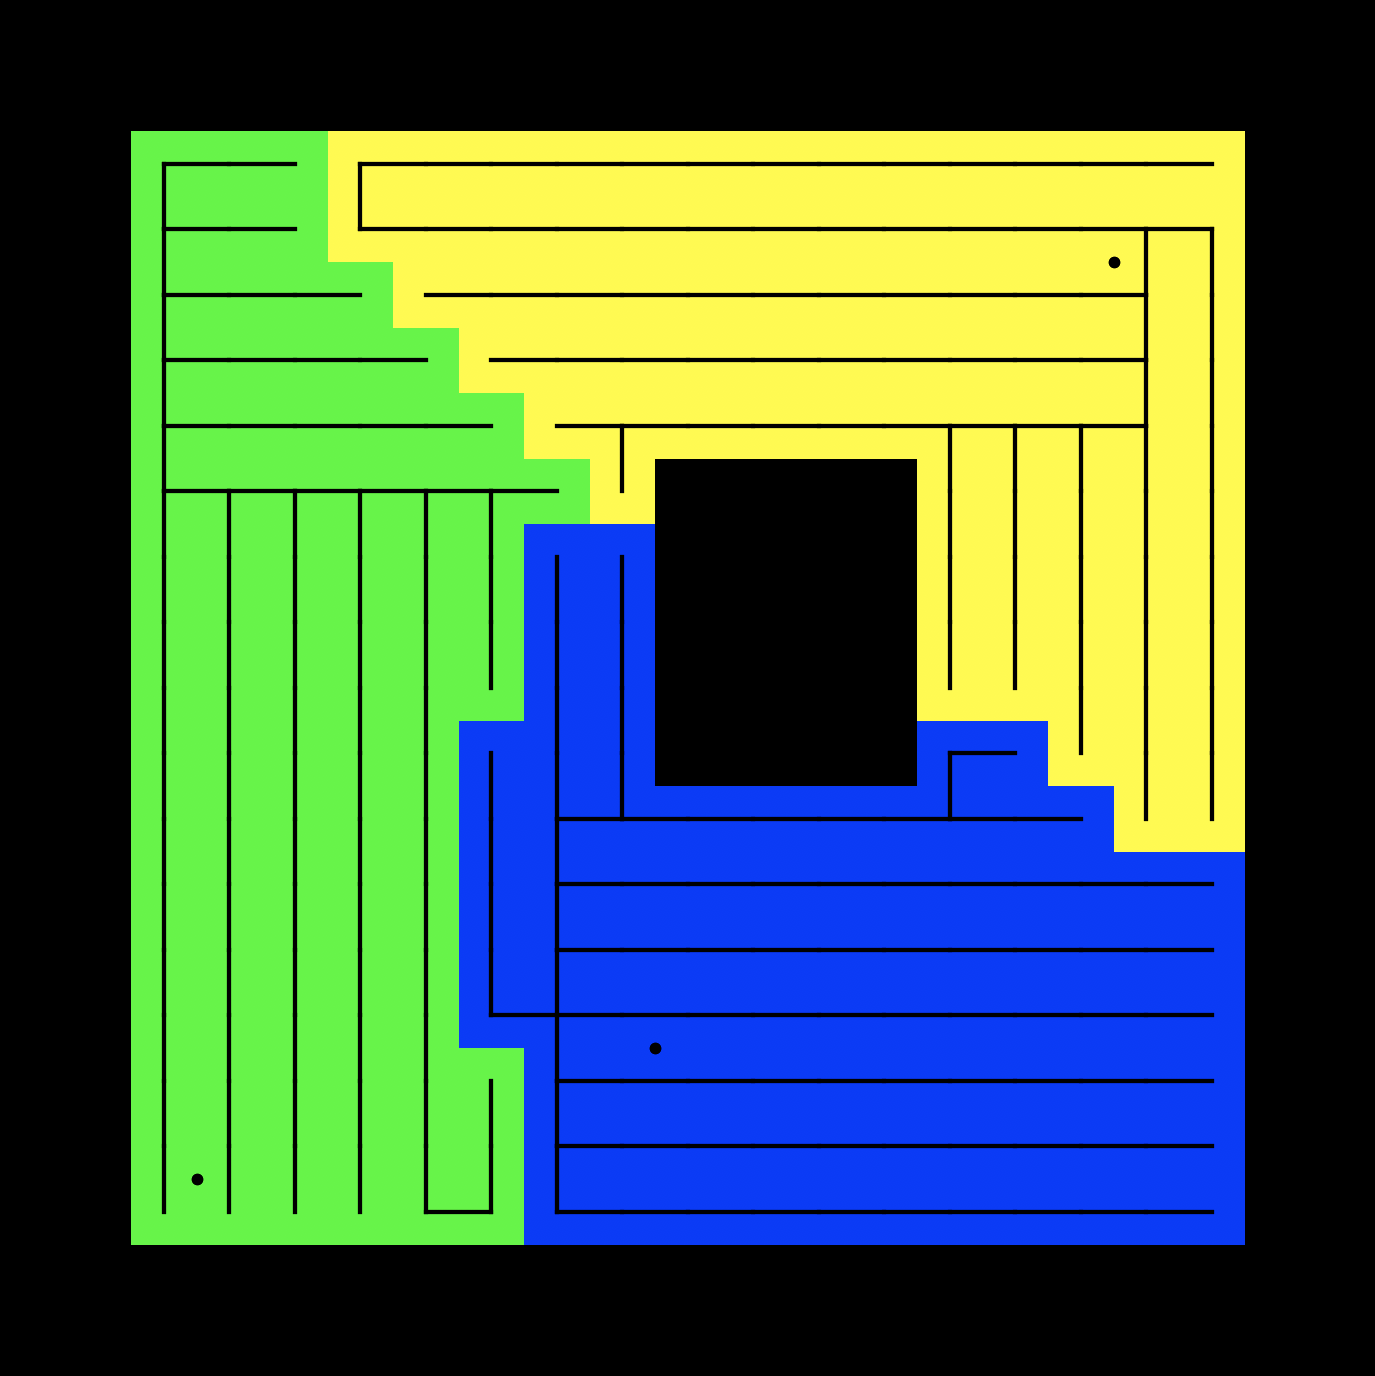
\includegraphics[width=0.8\columnwidth]{figure_mst.png}
	\caption{Spanning trees for each of the three regions.}
	\label{fig:mst}
\end{figure}

\subsection{Path Following}
To calculate movement instructions to give to each robot, we first break the required path down into the key poses. We define the key poses to be where a change of direction is required. For each robot, rather than estimate which key pose it should be heading for based on where it is, we mandate that it heads to each pose sequentially, and only moves on to the next one, once it has reached its required pose. The reason for this is that a little variation in the robot's estimation of its pose could cause it to appear to be on a different section of the required trajectory, and this could lead to somewhat random movement. For each pose that is the current target we calculate the required velocity and then apply feedback linearization to get the necessary control inputs to navigate the robot.



\subsection{Results}
To establish how well this navigation algorithm performs, particularly when it works off predictions of the robots' locations obtained through the localisation algorithm, we first obtained a base performance where we assumed perfect localisation by using ground truth values. We wanted the robots to move as fast as they safely could, so that they would cover the world in the shortest time possible, whilst avoiding collisions and staying on their designated path.

Figure~\ref{fig:ground_truth} shows the rate at which a system using ground truths covered the map, and figure~\ref{fig:ground_truth_coverage} shows the paths that the robots took. We see that the robots had fairly equally sized regions, and completed covering their respective regions at roughly the same time.

We can compare this to the performance of the coverage algorithm when using the locations predicted by the localisation algorithm - both when using the multi-robot enhancement, and when not. We would expect to see that when we have more accurate localisation, our time to cover the world will be lower. With more accurate positioning, the robots will do a better job of staying on their path and will therefore spend less time duplicating coverage. Indeed, we see that when using our multi-robot localisation

\begin{figure}
	\centering
	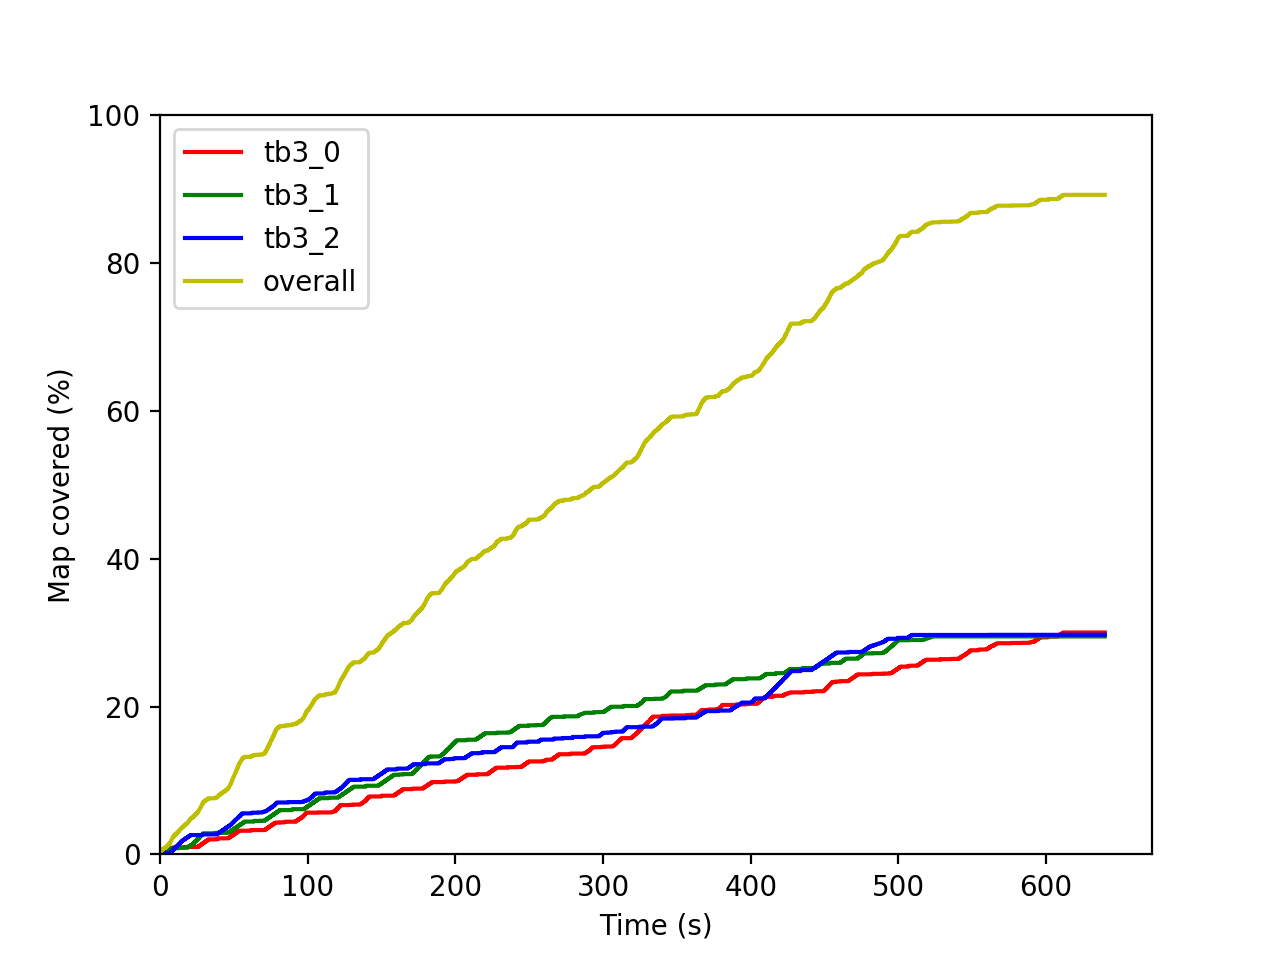
\includegraphics[width=\columnwidth]{ground_truth.png}
	\caption{Progression of world coverage with time.}
	\label{fig:ground_truth}
\end{figure}

\begin{figure}
	\centering
	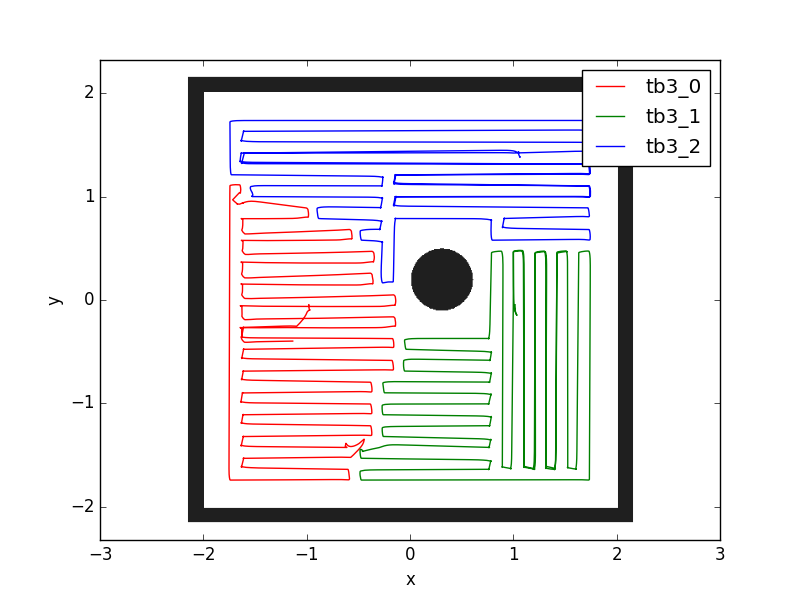
\includegraphics[width=\columnwidth]{ground_truth_coverage.png}
	\caption{Robots' paths to cover the world.}
	\label{fig:ground_truth_coverage}
\end{figure}

\begin{table}[h!]
  \begin{center}
    \caption{Time to cover 80\% of the map}
    \label{tab:table1}
    \begin{tabular}{|l|c|}
      \hline
      \textbf{Number of Robots} & \textbf{Time (s)} \\
      \hline
      1 & 0\\
      2 & 0\\
      3 & 0\\
      4 & 0\\
      5 & 0\\
      \hline
    \end{tabular}
  \end{center}
\end{table}


\section{Decentralised Navigation}
This section of the project was developed by Paul Durbaba (pd452). Trading of coverage regions was used to ensure that robots have different regions to cover, and a combination of the spanning tree approach with some extra navigation and collision avoidance was used for navigation of these regions.

\subsection{Region Trading}
The region trader works by using an auction of grid cells available. When two robots are within range of each other, they start a trade, with all cells previously owned by either for sale. All robots start out believing that they own the entire world. Robots first purchase the position they are currently at (the trade is aborted if one of the robots is outside of the for sale region), and then expand outwards from this using breadth first search.

To avoid a robot getting trapped in a corner, a robot is able to purchase cells already purchased by the other robot should it run out of cells to buy, which introduces two complications: First, it is possible that buying a cell owned by the other robot would split that robot's region in two. Second, it is now possible for one robot to buy the position of the other, and hence the other robot ends up outside it's own region.

To deal with the first, I example the 3x3 grid around the other robot's previously owned cell, to ensure that all cells owned by that robot in this 3x3 are connected. The second problem is dealt with by making robots navigate using RRT back to their region if they find themselves outside it.

This region trading algorithm converges (meaning that no robots have intersecting regions) in about 10 random trades with 3 robots. In general, the algorithm would require every robot to meet with every other robot to guarantee convergence, thus taking $O(n^2)$ random trials, which I verified using a script to count the number of trials required for different numbers of robots. However, in practice this is not so much of a problem because robots trade regions with nearby robots, which are the robots that would otherwise have overlapping regions.

\subsection{Navigation}
Robots use the MST approach to navigate within their own regions, resorting to RRT should they find themselves outside their region. There is a two phase collision avoidance system used to prevent collisions both with the world and with other robots, that operates using LIDAR and range/bearing measurements only.

In the first phase of collision avoidance, robots slow down and change their bearing slightly to avoid colliding with the obstacle. This uses the front left / front right LIDAR sensors for the world, and with other robots, the bearing is adjusted to rotate away from the imaginary line that would connect the two robots.

The second phase, when the current path is certain to result in a collision, is to drop the current path and revert to rule based navigation until the robot has rotated sufficiently that they would no longer collide if they moved forward. This can then result in the robot navigating outside it's region and having to use RRT to re-enter it.

\begin{figure}
	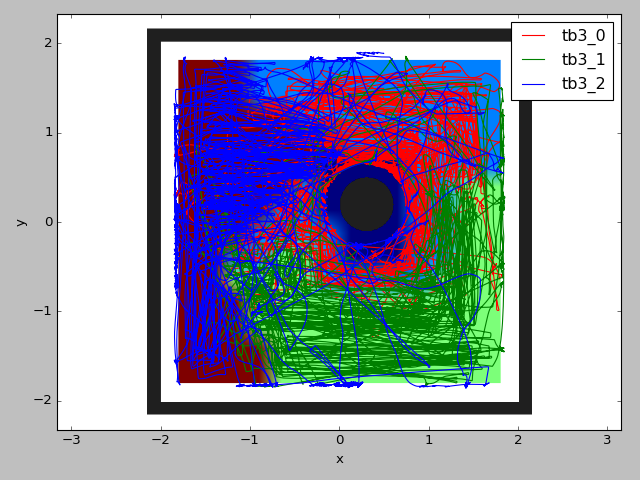
\includegraphics[width=\columnwidth]{dec_t2_cover.png}
	\caption{Robot trajectories within regions after 8000 seconds}
    \label{fig:decCover}
\end{figure}


Figure \ref{fig:decCover} shows the resulting trajectories of the robots within their regions, based on outputting each robot's position 10 times per second. By counting how often they fall inside their regions, robots 0 (red line on blue) ,1 (green on green) and 2 (blue line on brown) spend 84\%, 91\% and 70\% of their time within their own regions respectively.

\begin{figure}
	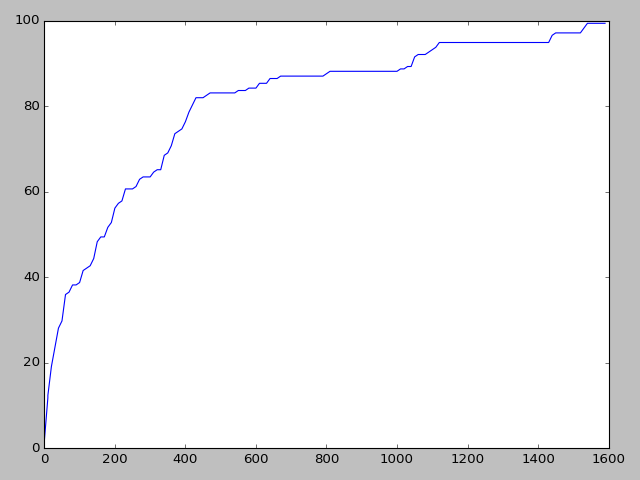
\includegraphics[width=\columnwidth]{dec_t2_line_percent.png}
	\caption{Coverage (percent of region cells out of 178) / Time (seconds)}
    \label{fig:decLine}
\end{figure}

Figure \ref{fig:decLine} shows the number of grid cells covered over time, showing that after 500 seconds the robots are able to cover 80\% of the world. The robots are programmed to move very slowly (0.15 m/s), but even at that speed localization errors will result in some cells being missed on some laps of the MST. However, after 1600 seconds each of the grid cells is able to be covered.

\section{Evaluation}
\section{Conclusions}
\begin{thebibliography}{9}
\bibitem{prorok} A. Prorok, Models and Algorithms for Ultra-Wideband Localization in Single- and Multi-Robot Systems. 2013.
\bibitem{darp} A. Kapoutsis et al. DARP: Divide Areas Algorithm for Optimal Multi-Robot Coverage Path Planning
\end{thebibliography}
\end{document}